\documentclass[a4paper,11pt]{article}
\usepackage{a4wide}
\usepackage{fullpage}
\usepackage[utf8x]{inputenc}

\usepackage[light,math]{anttor}
\usepackage[T1]{fontenc}

%\usepackage[slovene]{babel}
%\selectlanguage{slovene}
\usepackage[toc,page]{appendix}
\usepackage[pdftex]{graphicx} 

\usepackage{lmodern}
\usepackage{amsmath}
\usepackage{amssymb}
\usepackage{amsthm}
\usepackage{amsfonts}
\usepackage{mathtools}
\usepackage{enumitem}
\usepackage{amsfonts}
\usepackage{setspace}
\usepackage{color}
\definecolor{light-gray}{gray}{0.95}
\usepackage{listings} 
\usepackage{hyperref}
\usepackage[english, croatian, slovene]{babel}

\renewcommand{\baselinestretch}{1.2} 
\renewcommand{\appendixpagename}{Priloge}


\title{Algoritmi \\
\textbf{Domača naloga 2} }
\author{Sara Bizjak  |  27202020}
\date{April 2021}

%%%%%%%%%%%%%%%%%%%%%%%%%%%%%%%%%%%%%%%%%%%%%%%%%%%%%%%%%%%%%%%%%%%%%%%%%%%%%%%%%%%%%%%%%%%%%%%%%%%%%%%%%%%%%%%%%%%%%%%%%%%%%%%%%

\begin{document}

\maketitle

%%%%%%%%%%%%%%%%%%%%%%%%%%%%%%%%%%%%%%%%%%%%%%%%%%%%%%%%%%%%%%%%%%%%%%%%%%%%%%%%%%%%%%

\section*{Problem 1 - Ujemanje vzorcev}

%%%%%%%%%%%%%%%%%%%%%%%%%%%%%%%%%%%%%%%%%%%%%%%%

\subsection*{A del:}

Za podan vzorec $s$ izračunamo KMP preponsko funkcijo $\pi$.
$$s = \texttt{ababbabbabbabababbabb} $$
Podan imamo niz $s$ dolžine $n$. 
Preponska funkcija je definirana kot seznam $\pi$ dolžine $n$, kjer je $\pi[i]$ dolžina najdaljše ustrezne predpone podniza $s[0 \ldots i]$, kar je tudi pripona tega podniza.
Ustrezna predpona niza je definirana kot predpona, ki ni enaka samemu nizu. Po definiciji velja

$$
    \pi [0] = 0,
$$

\noindent
definicijo predponske funkcije pa matematično zapišemo kot

$$
    \pi [i] = \max_{k = 0, \ldots, i} \{ k : s [ 0 \ldots k - 1 ] = s [ i - (k - 1) \ldots i ] \}
$$

\noindent
Koda za iskanje KMP preponske funkcije $\pi$:

\begin{lstlisting}[language=Python]
def prefix_function(s):
    n = len(s)
    pi = [0 for i in range(n)]
    for i in range(1, n):
        k = pi[i - 1]
        while k > 0 and s[i] != s[k]:
            k = pi[k - 1]
        if s[i] == s[k]:
            k = k + 1
        pi[i] = k
    return pi
\end{lstlisting}

\noindent
Program vrne \texttt{$\pi = [0, 0, 1, 2, 0, 1, 2, 0, 1, 2, 0, 1, 2, 3, 4, 3, 4, 5, 6, 7, 8]$}.

%%%%%%%%%%%%%%%%%%%%%%%%%%%%%%%%%%%%%%%%%%%%%%%%

\subsection*{C del:}

Sestavimo končni avtomat za iskanje \texttt{asparagina (AAU, AAC)} in \texttt{metionina (AUG)}. 
Napišemo program, ki genom prebere in s pomočjo avtomata vrne lokacija vseh pojavitev želenih amino kislin.
Z drugimi besedami, iščemo končni avtomat, ki bo v genomu poiskal vse pojavitve vzorcev \texttt{AAUAUG} in \texttt{AACAUG}.
\\
\\
Avtomat predstavimo kot:
\begin{itemize}
    \item množica stanj $Q = \{ q_0, q_1, q_2, q_3, q_4, q_5, q_6 \}$
    \item začetno stanje $q_0$
    \item množica sprejemajočih stanj $A = \{ q_6 \}$
    \item vhodna abeceda $ \Sigma = \{ A, U, C, G\}$
    \item prehodna funkcija $ \delta$
\end{itemize}

\noindent
Tabela prehodne funkcije $ \delta$:
\\

\begin{table}[ht!]
    \begin{center}
        \scalebox{1.2}{%
        \begin{tabular}{c||cccc}
        \texttt{stanje / vhod} & \ \texttt{A}   & \ \texttt{U}    & \ \texttt{C}    & \ \texttt{G}    \\[0.2cm]  \hline \hline 
        $q_0$        & \ \ $q_1$ & \ \ $q_0$ & \ \ $q_0$ & \ \ $q_0$ \\[0.15cm] \hline
        $q_1$      & \ \ $q_2$ & \ \ $q_0$ & \ \ $q_0$ & \ \ $q_0$ \\[0.15cm] \hline
        $q_2$         & \ \ $q_2$ & \ \ $q_3$ & \ \ $q_3$ & \ \ $q_0$ \\[0.15cm]  \hline
        $q_3$         & \ \ $q_4$ & \ \ $q_0$ & \ \ $q_0$ & \ \ $q_0$ \\[0.15cm]  \hline
        $q_4$         & \ \ $q_2$ & \ \ $q_5$ & \ \ $q_0$ & \ \ $q_0$ \\[0.15cm]  \hline
        $q_5$         & \ \ $q_1$ & \ \ $q_0$ & \ \ $q_0$ & \ \ $q_6$ \\[0.15cm] \hline
        $q_6$         & \ \ $q_1$ & \ \ $q_0$ & \ \ $q_0$ & \ \ $q_0$ \\[0.15cm]
        \end{tabular}}
    \end{center}
\end{table}

\begin{figure}[ht!]
    \centering
    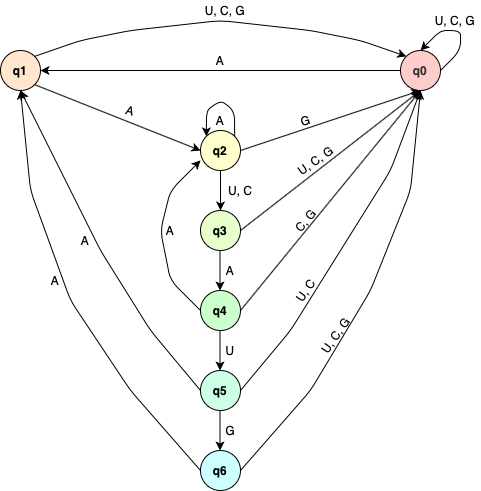
\includegraphics[width=120mm]{tranzicije.png}
    \caption{Grafični prikaz končnega avtomata za iskanje pojavitev vzorcev \texttt{AAUAUG} in \texttt{AACAUG}.}
\end{figure}

\newpage
\noindent
Napišemo še program, ki prebere genom in s pomočjo zgoraj generiranega avtomata vrne lokacije vseh pojavitev želenih aminokislin, tj. vzorcev \texttt{AAUAUG} in \texttt{AACAUG}.
Koda in primer sta dostopna v pythonovi datoteki \texttt{dn2\_tools.py}.
\\
\\
\noindent
Output priloženega primera iz datoteke \texttt{generated\_genome.txt} je:
\\
\noindent
[(87, 92), (741, 746), (2601, 2606), (5802, 5807), (12686, 12691), (13491, 13496), (16546, 16551), (20695, 20700), (22791, 22796), (27087, 27092), (29068, 29073), (32418, 32423), (33616, 33621), (35313, 35318), (38418, 38423), (38512, 38517), (39254, 39259), (40316, 40321), (47611, 47616), (48406, 48411), (49426, 49431), (49480, 49485), (50297, 50302), (52819, 52824), (56505, 56510), (59779, 59784), (60732, 60737), (64416, 64421), (66670, 66675), (69173, 69178), (70362, 70367), (71221, 71226), (71765, 71770), (72389, 72394), (72727, 72732), (73763, 73768), (77177, 77182), (77403, 77408), (77613, 77618), (79836, 79841), (83899, 83904), (84438, 84443), (84946, 84951), (85516, 85521), (90810, 90815), (95465, 95470), (96221, 96226), (96797, 96802), (98347, 98352), (99256, 99261)]
.

%%%%%%%%%%%%%%%%%%%%%%%%%%%%%%%%%%%%%%%%%%%%%%%%%%%%%%%%%%%%%%%%%%%%%%%%%%%%%%%%%%%%%%%%%%%%%%%%

\section*{Problem 2 -- IP posredovanje in vEB drevesa}

\subsection*{A del:}

\noindent
Uporabimo Mojstrov teorem in izračunamo časovno zahtevnost operacije \texttt{vEB-Tree-Successor} vEB drevesa.
Pokažemo še, da je časovna zahtevnost te operacije enaka $\mathcal{O}(\log \log M)$, kjer je $M$ velikost univerzuma. Predpostavimo, da je $M$ oblike $2^k$.
\\
\\
Spomnimo se najprej Mojstrovega izreka, ki pravi

\begin{align}\label{master}
T(n) = a \cdot T \left( \frac{n}{b} \right) + \mathcal{O}(n^c) = 
    \begin{dcases*} 
        \mathcal{O}(n^c) \ ; \ a < b^c \\ 
        \mathcal{O}(n^c \log n) \ ; \ a = b^c \\ 
        \mathcal{O}(n^{\log_b a}) \ ; \ a > b^c  
    \end{dcases*} 
\end{align}

\noindent
Vsi elementi, s katerimi se bomo ukvarjali, so števila v univerzalni množici $U = \{ 0, 1, \ldots, M - 1\}, \ |U| = M = 2^k$.
Korensko vozlišče eVB drevesa $T$ nad množico $U$ hrani seznam \texttt{T.children} dolžine $\sqrt{M}$, kjer je \texttt{T.children[i]} poddrevo z vrednostmi $\{ i \cdot \sqrt{M}, \ldots, (i + 1) \cdot \sqrt{M} - 1\}$.
Poleg tega drevo $T$ hrani še vrednosti \texttt{T.min} in \texttt{T.max} ter pomožno eVB drevo \texttt{T.aux}, kjer

\begin{itemize}
    \item \texttt{T.min} najmanjša vrednost, ki je trenutno v drevesu,
    \item \texttt{T.max} največja vrednost, ki je trenutno v drevesu,
    \item \texttt{T.children[i]} hrani (ostale) vrednosti $x$ za $i =  \lfloor \frac{x}{\sqrt{M}} \rfloor$,
    \item \texttt{T.aux} vsebuje vrednosti $j$ samo takrat, ko \texttt{T.children[j]} ni prazen.
\end{itemize}

\noindent
Za prazno drevo $T$ definiramo \texttt{T.max} = $- 1$ in \texttt{T.min} = $M$.
\\
\\
Algoritem, ki išče naslednika števila $x$ v drevesu $T$ poteka na naslednji način:
\begin{itemize}

    \item Če $x < \texttt{T.min}$, smo z iskanjem končali in naslednik za $x$ je $\texttt{T.min}$.
    \item Če $x \geq \texttt{T.max}$, potem naslednik za $x$ ne obstaja in vrnemo $M$.
    \item Sicer definirajmo $i = \frac{x}{\sqrt{M}}$.

        \begin{itemize}
            \item Če je $x < \texttt{T.children[i].max}$, je naslednik vsebovan v $\texttt{T.children[i]}$.
            \item Če je $x \geq \texttt{T.children[i].max}$, je naslednik vsebovan v $\texttt{T.aux}$. Tako dobimo indeks $j$ prvega poddrevesa, ki vsebuje naslednik elementa $x$. Naslednik $x$ je v tem primeru $\texttt{T.children[j].min}$.
        \end{itemize}

\end{itemize}

\noindent
Algoritem v vsakem primeru najprej porabi $\mathcal{O}(1)$ in se potem lahko izvede še na poddrevesu velikosti $\sqrt{M}$, kar vzame $\mathcal{O}(\sqrt{M}) = \mathcal{O} \left( M^{\frac{1}{2}} \right)$, 
torej $\mathcal{O} \left( 2^{\frac{k}{2}} \right)$.
\\
Sledi
$$
T(k) = T \left( \frac{k}{2} \right) + \mathcal{O}(1)
$$
in po izreku \ref{master} so konstante $a, b$ in $c$ enake: 
$$ a = 1, \  b = 2, \ c = 0  \ \text{in zato velja} \ a = b^c,$$
torej
$$
T(k) = \mathcal{O}(\log k) = \mathcal{O}(\log \log M)
$$

%%%%%%%%%%%%%%%%%%%%%%%%%%%%%%%%%%%%%%%%%%%%%%%%

\subsection*{B del:}

Naivni pristop pri štetju bitov s pomočjo povzetkovne tabele z Lulea algoritmom potrebuje tri pomnilniške reference.
Razložimo, kako lahko prva dva stolpca združimo v enega.
\\
V Luela algoritmu na prvih dveh pomnilniških referencah hranimo pozvetkovno tabelo $P$ in bitno tabelo $B$ ločeno. 
Tabela $P$ je enake dolžine kot je število kosov v bitni tabeli, tabela $B$ pa je sestavljena iz kosov določene dolžine.
Označimo z $M$ tabelo z združenim dostopom. $M$ zgradimo tako, da $P$ in $B$ prepletemo tako, da pred $i-$ti kos v $B$ shranimo $i-$ti element povzetkovne tabele.
Za vsak $i$ poznamo zgornjo mejo za $P(i)$, zato v $M$ tej vrednosti namenimo le toliko bitov prostora, kot ga potrebuje.
\\
Natančneje, 
v enem dostopu do pomnilnika je možno dobiti največ $64$ bitov in ker je bitno polje dolgo največ $2^{16}$, števila v tabeli $P$ porabijo največ $16$ bitov. 
Zato je potrebno kose v tabeli $B$ zmanjšati na $48$ bitov, da bodo skupaj s pripradajočim številom tabele $P$ zavzeli največ $64$ bitov, torej bomo lahko do elementov združene tabele $M$ res dostopali s samo enim dostopom.

%%%%%%%%%%%%%%%%%%%%%%%%%%%%%%%%%%%%%%%%%%%%%%%%

\subsection*{C del:}

\begin{figure}[ht!]
    \centering
    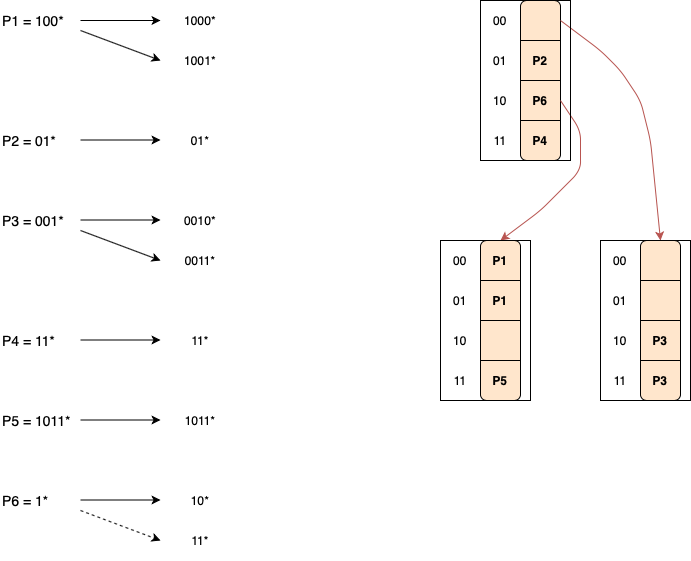
\includegraphics[width=110mm]{fixed_stride.png}
    \caption{\textit{Fixed stride} številsko drevo s stride velikostjo $2$.}
\end{figure}

%%%%%%%%%%%%%%%%%%%%%%%%%%%%%%%%%%%%%%%%%%%%%%%%%%%%%%%%%%%%%%%%%%%%%%%%%%%%%%%%%%%%%%%%%%%%%%%%

\section*{Problem 3 -- Kompaktne podatkovne strukture}

\noindent
Podano imamo drevo.

\begin{figure}[ht!]
    \centering
    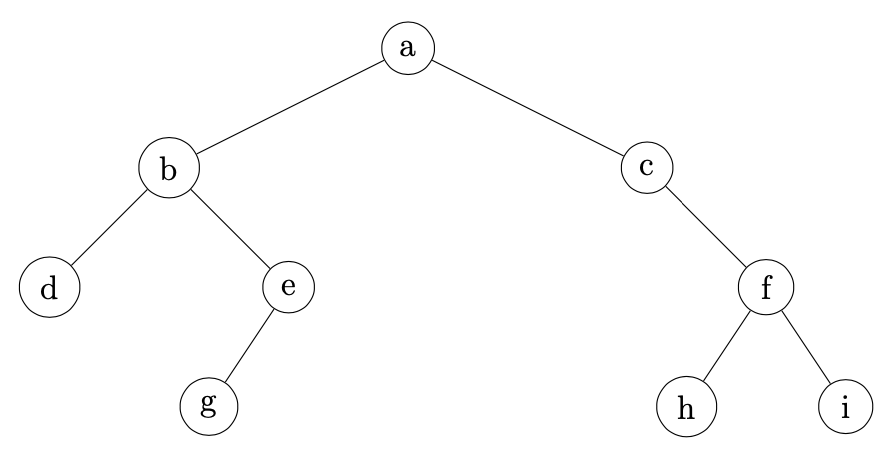
\includegraphics[width=120mm]{drevo3.png}
    \caption{Slika podanega drevesa.}\label{drevo}
\end{figure}

\subsection*{A del:}
Predpostavimo, da je drevo na sliki \ref{drevo} ordinalno in ga zapišemo v obliki BP in LOUDS.
\begin{itemize}
    \item \texttt{BP: ((()(()))((()())))}
    \item \texttt{LOUDS: 1011011010010110000}
\end{itemize}

%%%%%%%%%%%%%%%%%%%%%%%%%%%%%%%%%%%%%%%%%%%%%%%%

\subsection*{B del:}
Predpostavimo, da je drevo na sliki \ref{drevo} kardinalno in ga zapišimo b obliki BP in LOUDS.
\begin{itemize}
    \item \texttt{BP: (((()())((()())()))(()((()())(()()))))}
    \item \texttt{LOUDS: 10110110010000100110000000000}
\end{itemize}

%%%%%%%%%%%%%%%%%%%%%%%%%%%%%%%%%%%%%%%%%%%%%%%%

\subsection*{C del:}
Za kardinalno drevo v obliki BP zgradimo \texttt{rmM-drevo} za $b = 8$.
\\
\texttt{BP: (((()())((()())()))(()((()())(()()))))}

\begin{figure}[ht!]
    \centering
    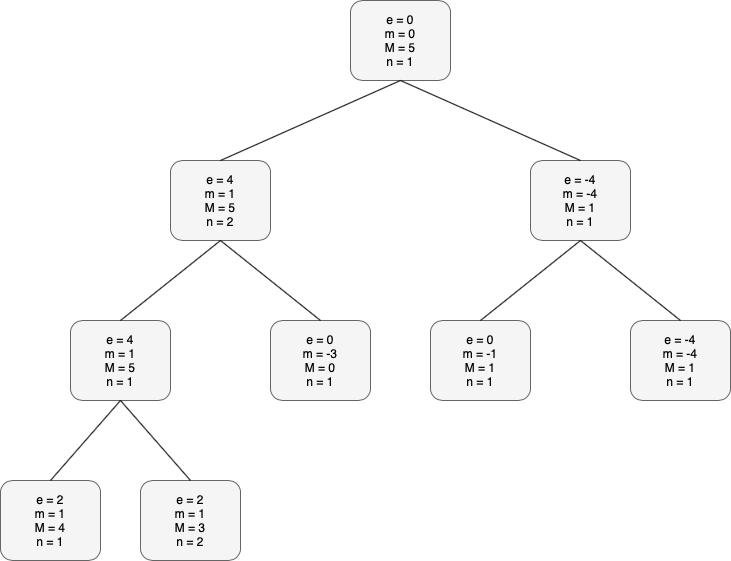
\includegraphics[width=150mm]{graff.png}
    \caption{rmM-drevo za $b = 8$.}
\end{figure}

%%%%%%%%%%%%%%%%%%%%%%%%%%%%%%%%%%%%%%%%%%%%%%%%

\newpage
\subsection*{D del:}
Napišemo psevdo-koda za funkcijo \texttt{Izberi(T, i)}, ki vrne $i$-ti element v razširjenem iskalnem dvojiškem drevesu $T$.
Drevo $T$ v vsakem vozlišču hrani moč levega poddrevesa $|L|$.
\\
Funkcijo definiramo rekurzivno. V funkciji z \texttt{L} in \text{D} označimo levo in desno poddrevo, z \texttt{|L|} in \texttt{|D|} pa velikost levega in desnega poddrevesa. \texttt{T.koren} vrne koren drevesa $T$.

\begin{lstlisting}[language=Python]

Izberi(T, i):
    // i-ti element je korensko vozlisce //
    ce i = |L| + 1:     
        vrni T.koren 
    // i-ti element je v levem poddrevesu //
    ce i < |L| + 1:    
        vrni Izberi(L, i)
    // i-ti element je v desnem poddrevesu //
    sicer:      
        vrni Izberi(D, i - |L| - 1)

\end{lstlisting}

%%%%%%%%%%%%%%%%%%%%%%%%%%%%%%%%%%%%%%%%%%%%%%%%%%%%%%%%%%%%%%%%%%%%%%%%%%%%%%%%%%%%%%%%%%%%%%%%

\newpage
\begin{thebibliography}{99}
    \bibitem -T.~H.~Cormen, C.~E.~ Leiserson, R.~L.~Rivest, C.~Stein, \emph{Introcustion to Algorithms}, third edition, [ogled 1.~4.~2021], dostopno na \url{edutechlearners.com/download/Introduction_to_algorithms-3rd%20Edition.pdf}.
\end{thebibliography}
    
\end{document}



\begin{table}[ht!]
    \begin{center}
        \begin{tabular}{c|cccc}
        stanje / vhod & \ $A$   & \ $U$   & \ $C$   & \ $G$   \\ \hline
        $q_0$         & \ $q_1$ & \ $q_0$ & \ $q_0$ & \ $q_0$ \\ \hline
        $q_1$         & \ $q_2$ & \ $q_0$ & \ $q_0$ & \ $q_0$ \\ \hline
        $q_2$         & \ $q_2$ & \ $q_3$ & \ $q_3$ & \ $q_0$ \\ \hline
        $q_3$         & \ $q_4$ & \ $q_0$ & \ $q_0$ & \ $q_0$ \\ \hline
        $q_4$         & \ $q_2$ & \ $q_5$ & \ $q_0$ & \ $q_0$ \\ \hline
        $q_5$         & \ $q_1$ & \ $q_0$ & \ $q_0$ & \ $q_6$ \\ \hline
        $q_6$         & \ $q_1$ & \ $q_0$ & \ $q_0$ & \ $q_0$
        \end{tabular}
    \end{center}
\end{table}


\begin{figure}[ht!]
    \centering
    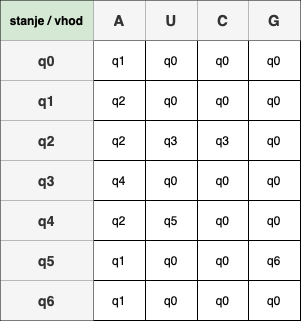
\includegraphics[width=70mm]{tabela.png}
    \caption{Tabela prehodne funkcije $ \delta$.}
\end{figure}